\documentclass[11pt,letterpaper]{article}
\usepackage[utf8]{inputenc}
\usepackage[left=1in,right=1in,top=1in,bottom=1in]{geometry}
\usepackage{amsfonts,amsmath}
\usepackage{graphicx,float}
\usepackage{esint}
\usepackage{csquotes}
% -----------------------------------
\usepackage{hyperref}
\hypersetup{%
  colorlinks=true,
  linkcolor=blue,
  citecolor=blue,
  urlcolor=blue,
  linkbordercolor={0 0 1}
}
% -----------------------------------
\usepackage[authordate,backend=biber]{biblatex-chicago}
\addbibresource{citation.bib}
% -----------------------------------
\usepackage{fancyhdr}
\newcommand\course{MATH-UA.0230, PHYS-UA 180\\Introduction to Fluid Dynamics}
\newcommand\hwnumber{6}                  % <-- homework number
\newcommand\NetIDa{Ryan Sh\`iji\'e D\`u} 
\newcommand\NetIDb{March 9th, 2023}
\pagestyle{fancyplain}
\headheight 35pt
\lhead{\NetIDa\\\NetIDb}
\chead{\textbf{\Large Worksheet \hwnumber}}
\rhead{\course}
\lfoot{}
\cfoot{}
\rfoot{\small\thepage}
\headsep 1.5em
% -----------------------------------
\usepackage{titlesec}
\renewcommand\thesubsection{(\arabic{section}.\alph{subsection})}
\titleformat{\subsection}[runin]
        {\normalfont\bfseries}
        {\thesubsection}% the label and number
        {0.5em}% space between label/number and subsection title
        {}% formatting commands applied just to subsection title
        []% punctuation or other commands following subsection title
% -----------------------------------
\setlength{\parindent}{0.0in}
\setlength{\parskip}{0.1in}
% -----------------------------------
\newcommand{\de}{\mathrm{d}}
\newcommand{\DD}{\mathrm{D}}
\newcommand{\pe}{\partial}
\newcommand{\mcal}{\mathcal}
%\newcommand{\pdx}{\left|\frac{\partial}{\partial_x}\right|}

\newcommand{\dsp}{\displaystyle}

\newcommand{\norm}[1]{\left\Vert #1 \right\Vert}
%\newcommand{\mean}[1]{\left\langle #1 \right\rangle}
\newcommand{\mean}[1]{\overline{#1}}
\newcommand{\inner}[2]{\left\langle #1,#2\right\rangle}

\newcommand{\ve}[1]{\boldsymbol{#1}}

\newcommand{\thus}{\Rightarrow \quad }
\newcommand{\fff}{\iff\quad}
\newcommand{\qdt}[1]{\quad \mbox{#1} \quad}

\renewcommand{\Re}{\mathrm{Re}}
\renewcommand{\Im}{\mathrm{Im}}
\newcommand{\E}{\mathbb{E}}
\newcommand{\lap} {\nabla^2}
\renewcommand{\div}{\nabla\cdot}

\newcommand{\csch}{\text{csch}}
\newcommand{\sech}{\text{sech}}


\newcommand{\hot}{\text{h.o.t.}}

\newcommand{\ssp}{\left.\qquad\right.}

\newcommand{\var}{\text{var}}
\newcommand{\cov}{\text{cov}}


\begin{document}

\section{Reynolds number for simple model for river flow}
[From \cite{Falkovich_18}, \S 1.4.3] 
We use a simple inclined plane as a model for river flow.
\begin{figure}[H]
    \centering
    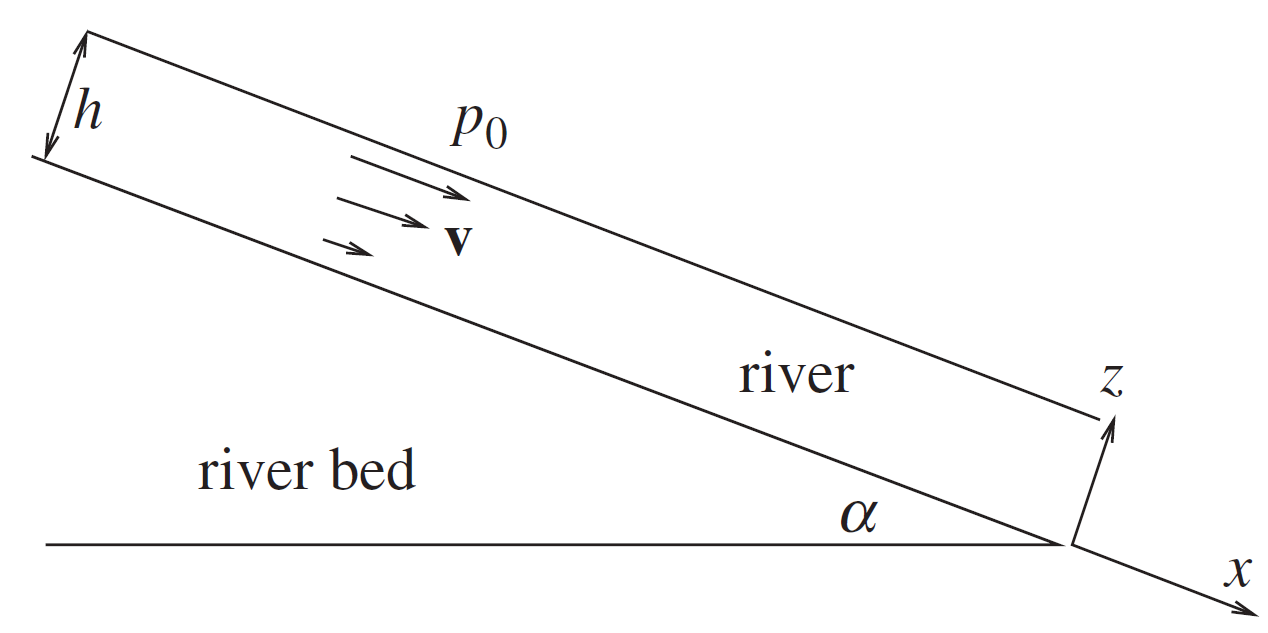
\includegraphics[width=0.55\textwidth]{figs/incline_river}
\end{figure}

In lecture you have the obtained the solution of:
\begin{align}
    p(z) &= p_0+\rho g(h-z)\cos\alpha,\\
    v(z) &= \frac{\rho g\sin\alpha}{2\eta}z(2h-z).
\end{align}

% \subsection{}
% Assume we have a steady solution to the Navier-Stokes equation, show $(\ve v\cdot\nabla)\ve v = 0$. This implies we have an effectively linear equation
% \begin{align}
%     -\nabla p+\eta\nabla^2\ve v+\rho\ve g = 0.
% \end{align}

% Write the equation for the $x$ and $z$ direction defines in the figure.

% \subsection{}
% What should be boundary condition be for $v$ and $p$ at the surface and at the bottom? Solve for them.

\subsection{}
Take the kinematic viscosity of water to be $\nu = \eta/\rho = 10^{-2}\;\text{cm}^2\text{s}^{-1}$. Calculate $\ve v$ at the surface for a rain puddle with thickness $h = 1\;\text{mm}$ on a slope $\alpha\sim 10^{-2}$.

\subsection{}
How about a slow plain rivers (like the Danube) with $h \sim 10\;\text{m}$ on a slope $\alpha\sim 10^{-4}$?

\subsection{}
Which speed is reasonable?

\subsection{}
The unrealistic high velocity for the river case above is because in reality rivers are turbulent. Calculate the Reynolds number for the two cases.

\section{Vorticity equation derivation}
Remember that we have the vector identity:
\begin{align}
    \ve v(\nabla\cdot\ve v) = \frac{1}{2}\nabla\ve v^2-\ve v\times\ve \omega.\label{eq:lamb_ident}
\end{align}
To obtain the vorticity equation, we need to take the curl of this. 

\subsection{}
Derive the vector identity:
\begin{align}
    \nabla\times(\ve a\times\ve b) &= \ve a(\nabla \cdot \ve{b}) \,-\, \ve{b}(\nabla {\cdot} \ve{a})+(\ve{b} {\cdot} \nabla) \ve{a} \,-\, (\ve{a} {\cdot} \nabla) \ve{b}.
\end{align}
Hint: remember we have
\begin{align}
    \epsilon_{ijk}\epsilon_{k\ell m} = \delta_{i\ell}\delta_{jm}-\delta_{im}\delta_{j\ell}.\label{eq:perm_prod_ident}
\end{align}

\subsection{}
Show that the compressible vorticity equation is
\begin{align}
    \frac{\pe\ve\omega}{\pe t}+(\ve v\cdot \nabla)\ve\omega = (\ve \omega\cdot \nabla)\ve v-\ve\omega\nabla\cdot\ve v
\end{align}
The incompressible version is an straightforward corollary. 

\section{Vorticity equation for compressible flows}
[From \cite{Vallis_17}, \S 4.2] Using mass-conservation for compressible flows:
\begin{align}
    \frac{\pe\rho}{\pe t}+\nabla\cdot(\rho\ve v) = 0
\end{align}
Obtain the alternative compressible vorticity equation:
\begin{align}
    \frac{\pe\tilde{\ve\omega}}{\pe t}+(\ve v\cdot \nabla)\tilde{\ve\omega} = (\tilde{\ve \omega}\cdot \nabla)\ve v
\end{align}
where
\begin{align}
    \tilde{\ve \omega} = \frac{\ve\omega}{\rho}.
\end{align}

\section{Fundamental solution to the heat equation}
\subsection{}
Self-similar solution from dimensional analysis. 

\subsection{}
Fundamental solution is the Green's function.




    
\vfill
\printbibliography


\end{document}